\subsubsection{CPU Usage} 

Charts on Figures \ref{fig:sequential_client_transport_cpu}, \ref{fig:parallel_client_transport_cpu}, \ref{fig:sequential_server_transport_cpu}, and \ref{fig:parallel_server_transport_cpu} represent the \gls{cpu} usage of clients and servers during ephemeral and persistent experiments.

\subsubsection*{Overall Clients CPU Usage}

Parallel requests with 32KiB and smaller payloads had a lower CPU usage when compared with sequential requests. Performing the former waits longer for each response to arrive, requiring more CPU time. Thus, small concurrent requests demands less CPU time.

Requests with 128KiB and larger payloads starts to shift this behavior. As larger payloads needs to be processed at the same time, it requires more CPU time than when processing one at a time. Therefore, when dealing with larger payloads, sequential requests spend less CPU time than parallel. 

\subsubsection*{QUIC's CPU Usage}

QUIC's CPU is greater than other protocols when requests are concurrent. It needs to deal with cryptography, sending and receiving of \gls{udp} packets, and maintaining internal QUIC state. Thus, requiring more CPU time.

\subsubsection*{Overall Server CPU Usage}

Server CPU usage remained roughly the same as client CPU usage. Requests and responses payloads have the same size. Therefore, clients and servers have to process the same amount of requests and responses, which explains why their CPU usage is so similar.

\clearpage

\begin{figure}[h!]
    \centering
    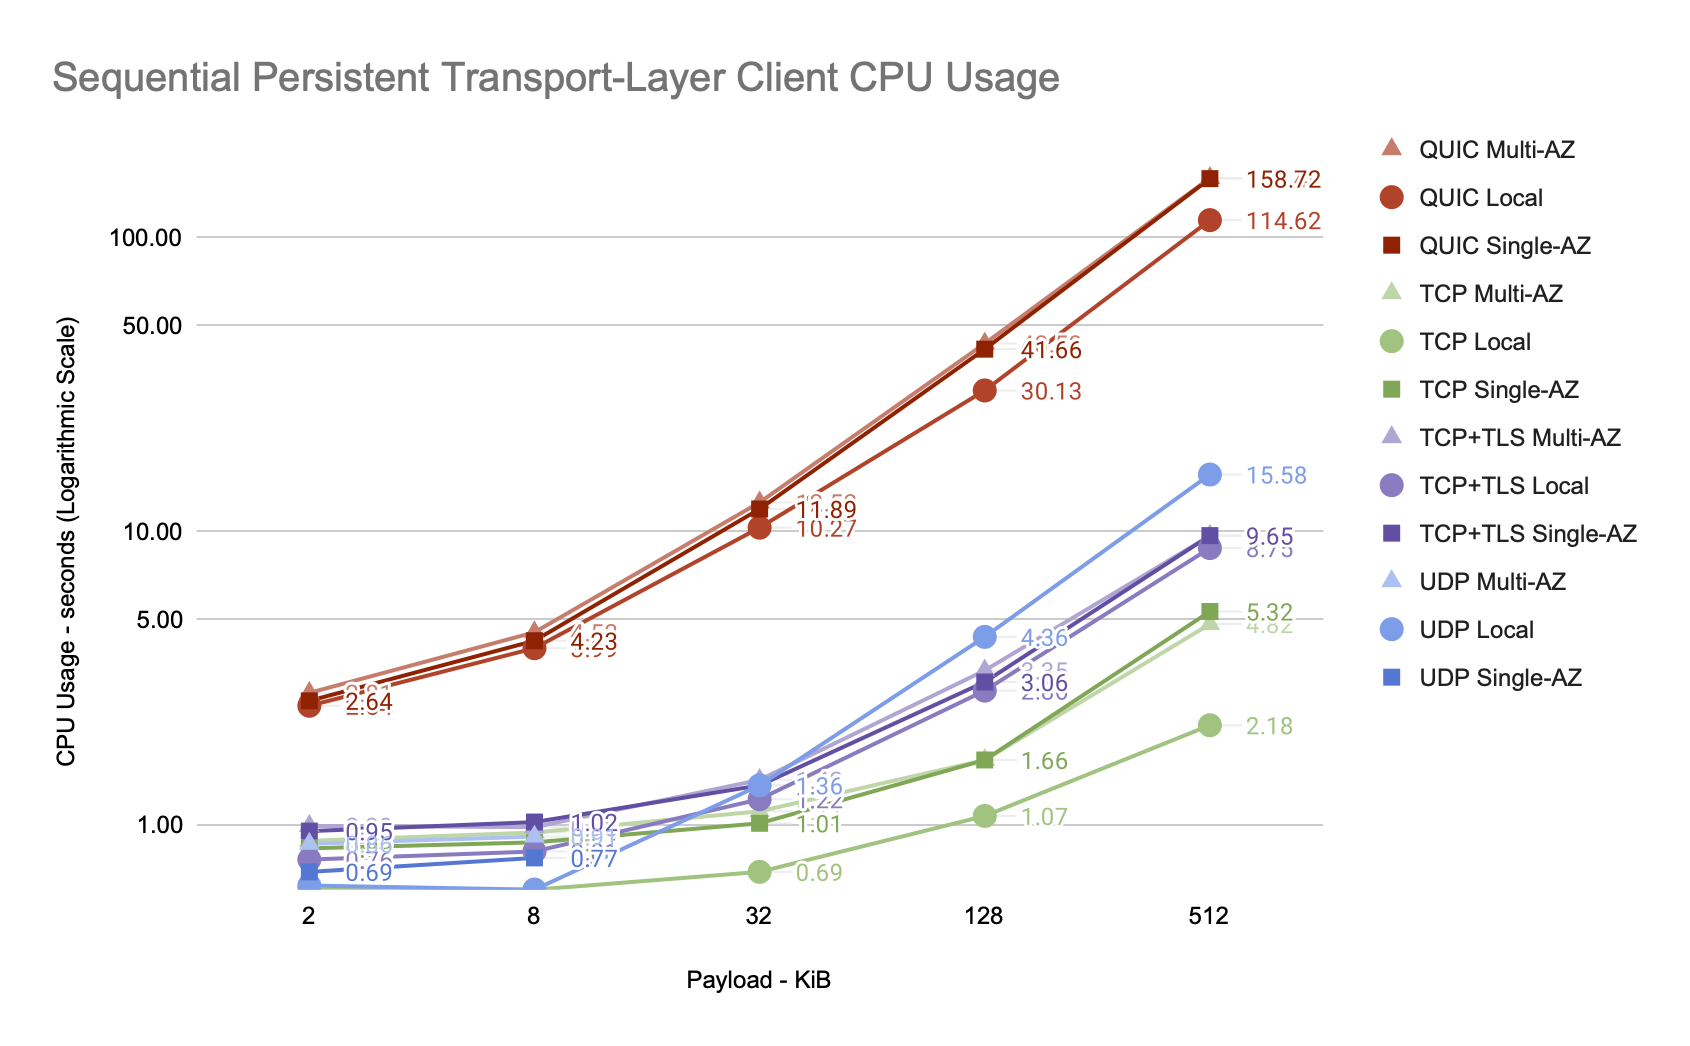
\includegraphics[width=\linewidth]{figures/charts/Sequential Persistent Transport-Layer Client CPU Usage.png}
    \caption{Sequential Persistent Transport-Layer Client CPU Usage}
    \label{fig:sequential_client_transport_cpu}
\end{figure}
\begin{figure}[h!]
    \centering
    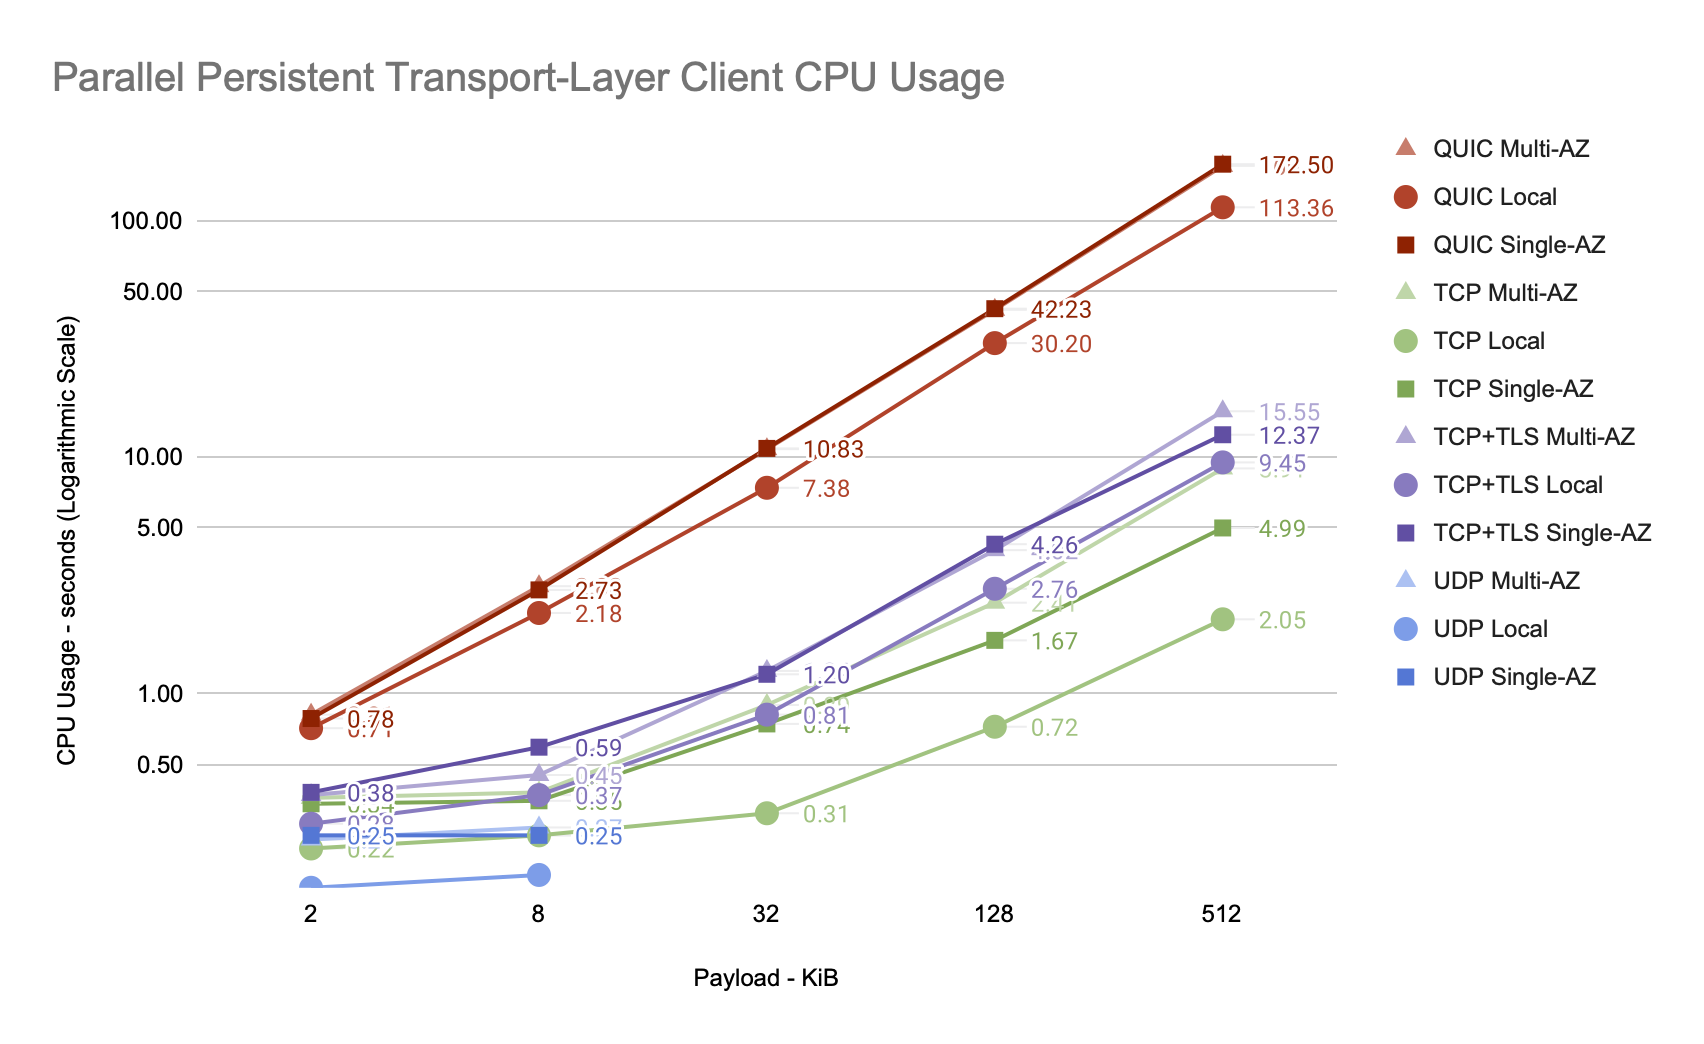
\includegraphics[width=\linewidth]{figures/charts/Parallel Persistent Transport-Layer Client CPU Usage.png}
    \caption{Parallel Persistent Transport-Layer Client CPU Usage}
    \label{fig:parallel_client_transport_cpu}
\end{figure}


\begin{figure}[h!]
    \centering
    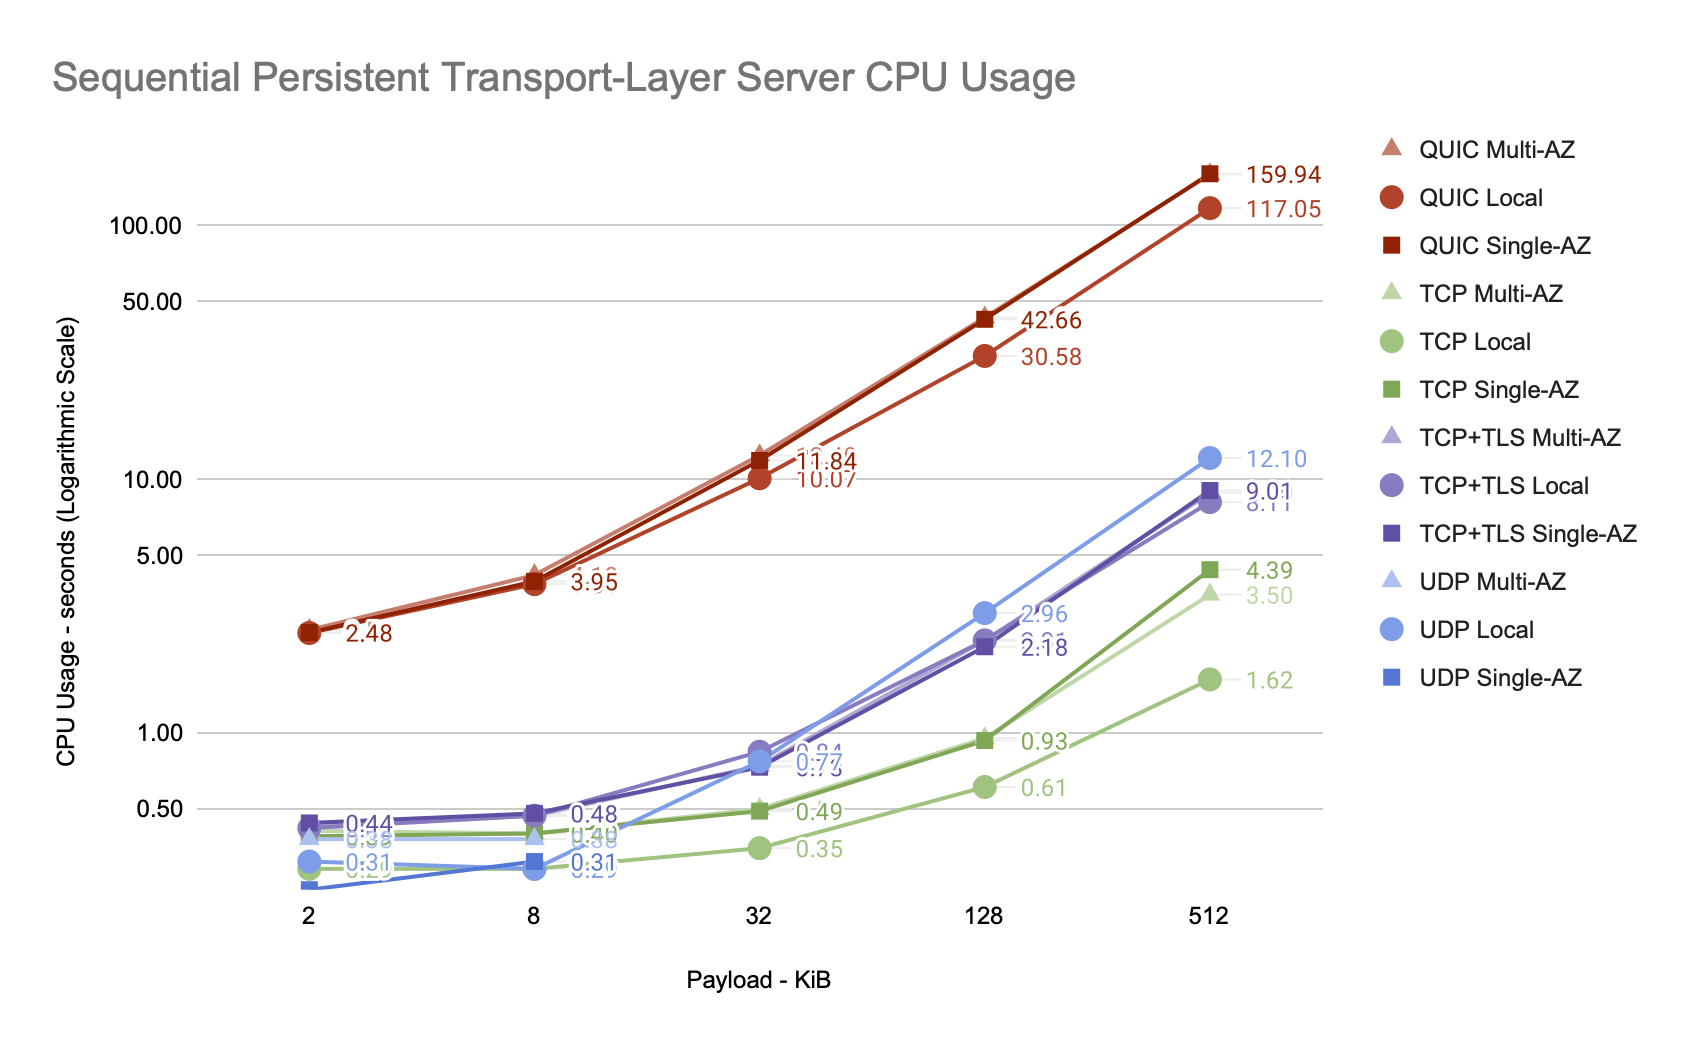
\includegraphics[width=\linewidth]{figures/charts/Sequential Persistent Transport-Layer Server CPU Usage.png}
    \caption{Sequential Persistent Transport-Layer Server CPU Usage}
    \label{fig:sequential_server_transport_cpu}
\end{figure}
\begin{figure}[h!]
    \centering
    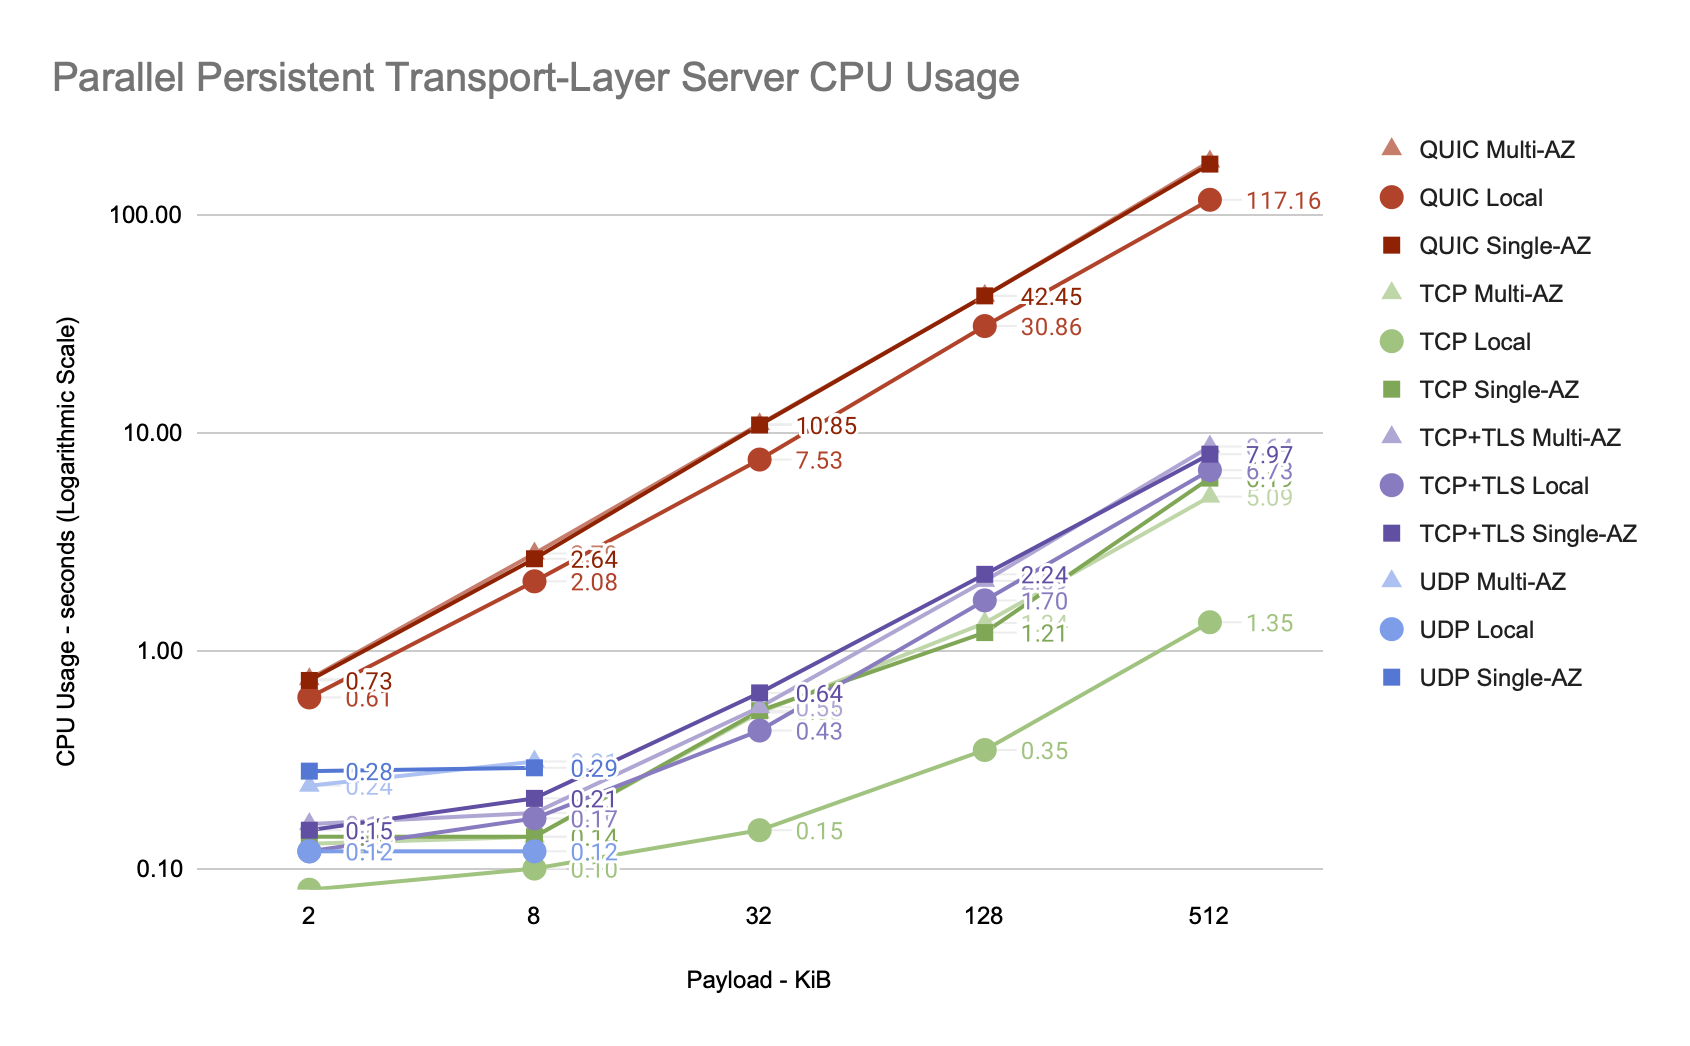
\includegraphics[width=\linewidth]{figures/charts/Parallel Persistent Transport-Layer Server CPU Usage.png}
    \caption{Parallel Persistent Transport-Layer Server CPU Usage}
    \label{fig:parallel_server_transport_cpu}
\end{figure}
